First, the uncertainty of the conditioning process, $\sigma_{con}$, was experimentally measured. This uncertanty appeares because, as we saw before, each fiber have to be conditioned, consisting in cutting and polishing it, before using. This is an individual task that can present a small dispersion, affecting the response of each individual fiber. It is an important measurement because this uncertainty will be present in the TRITIUM detector.

To measure it, it has to be taken into account that there is a bit of freedom in this system due to the position of the connectors which are fixed to the fiber ($1~\mm$ or less) which means that there is an additional uncertainty, $\sigma_{pos}$, in the measurement. Since both uncertainties are not related, the total measurement uncertainty can be calculated as a square sum, equation \ref{eq:TotalUncertaintyFiberCharacterization}.

\begin{equation}
\sigma_{t} = \sqrt{\sigma^2_{pos} + \sigma^2_{con} }
\label{eq:TotalUncertaintyFiberCharacterization}
\end{equation}

The uncertanty due to the fiber position are always presented in the measurements of this set up so, the only way to measure the uncertainty due to the conditioning process is to quantify the uncertainty in the fiber position and extract it to the total uncertainty, sum of both, using the equation \ref{eq:ConditioningUncertaintyFiberCharacterization}. To do so, two different experiments was designed, one where only the uncertainty in the fiber position are presented ($\sigma_{t} = \sigma_{pos}$), and other where both uncertainties are involved.

\begin{equation}
\sigma_{con} = \sqrt{\sigma^2_{tot} - \sigma^2_{pos} }
\label{eq:ConditioningUncertaintyFiberCharacterization}
\end{equation}

The test designed to measure $\sigma_{pos}$ consisted of prepare one fiber of each type (no clad, single clad and multiclad) using the conditioning process explained before. Then, fix each fiber in the set up, take a measurement by feeding the LED at an intensity of $0.1~\milli\ampere$ and remove this fiber to the set up (and also the connectors). These measurements is repeated ten times with the same fiber, fixing and removing it every time.

Ten different measurements for each fiber type is obtained with this test, the standard deviation of which is only due to the uncertainty in the position. The results is shown in Table \ref{tab:PositionStandardDeviation}, which was calculated using the equations \ref{eq:MeanAndStandardDesviation} and \ref{eq:RelativeStandardDesviation}.

\begin{equation}
Rel.~Std.~Des. = \frac{Std.Des.}{\bar{x}}
\label{eq:RelativeStandardDesviation}
\end{equation}

\begin{table}[htbp]
%%\centering
\begin{center}
\begin{tabular}{|c|c|c|c|c|}
\hline
Fiber type & Average ($\gamma$/ns) & Std. Des. ($\gamma$/ns) & Rel. Std. Des. (\%)\\
\hline \hline \hline
No Clad & $524.088 \pm 0.010$ & $17.65$ & $3.37$ \\ \hline
Single Clad & $1071.696 \pm 0.01$ & $9.07$ & $0.85$ \\ \hline
Multiclad & $949.930 \pm 0.026$ & $9.91$ & $1.04$ \\ \hline
\end{tabular}
\caption{Average and standard deviation (due to fiber position in setup) of photons per nanosecond that reach the PMT for $0.1~\milli\ampere$ LED intensity.}
\label{tab:PositionStandardDeviation}
\end{center}
\end{table}

As can be seen, the clad of the fiber reduces the uncertainty due to the position of the fiber, which means that it improves the uniformity of the fiber response. It can be also seen that the use of the clad greatly improves the collection efficiency of the fibers since both types of fibers with clad have collected more photons than the fiber without clad. It could be because photons are mainly collected in the core of the fiber and the interface created by this core and the surounding greatly affects the amount of photons collected. This interface can be much more controlled in the case of a single clad or multiclad fibers than in no clad fibers, where it is created between the core and the environment (air or water in the case of TRITIUM), where external conditions, such as the dirt in the room, can affect a lot.

We can also see that the use of a second clad slightly reduce the collection efficienciy. One possible reason for this is that, to add a second liner, the polystyrene core must be reduced proportionally.

%We don't achieve any improvement with the second clad, which means that the photons are mainly collected in the core of the fiber.

%A possible reason of that is because, in the case of no clad fibers, the state of the interface between the core and the environment (air or water in our case) is much more important than in the others, where the most important interface is the one created between the fiber core and the first clad, which could be the reason why the difference between the signals of single clad and multiclad fibers are too small.

It is also appreciate in the table that the error of the measurement, provided by the keithley and propagated to the average, is three times smaller than the standard deviation, so it was not taken into account any more.

%In addition to the $\sigma_{pos}$ measurement, we have measured the number of photons collected by each type of fiber in the same situation, which is higher for single clad and even higher for multiclad. It means that the clad has an appreciable effect on the fiber collection efficiency and it could be a possible point to futur studies.

The second experiment, in which both uncertainties are involved, consists of preparing ten different samples of each fiber type (using the conditioning process) and measuring each fiber under the same conditions as the previous test. This measurement was done for four different LED emission intensities ($0.05$, $0.1$, $0.15$ and $0.2~\milli\ampere$) to reduce possibles mistakes.

The case of no clad fibers is shown in Figure \ref{fig:10samplesNC}, where it can be seen that, indeed, although each fiber shows a very linear trend with the amount of photons that it collects, a dispersion in the fiber response is clearly seen in each figure. Similar results were obtained for single clad and multiclad fibers, shown in figures \ref{subfig:10samplesSC} and \ref{subfig:10samplesMC} respectively.

\begin{figure}[h]
\centering
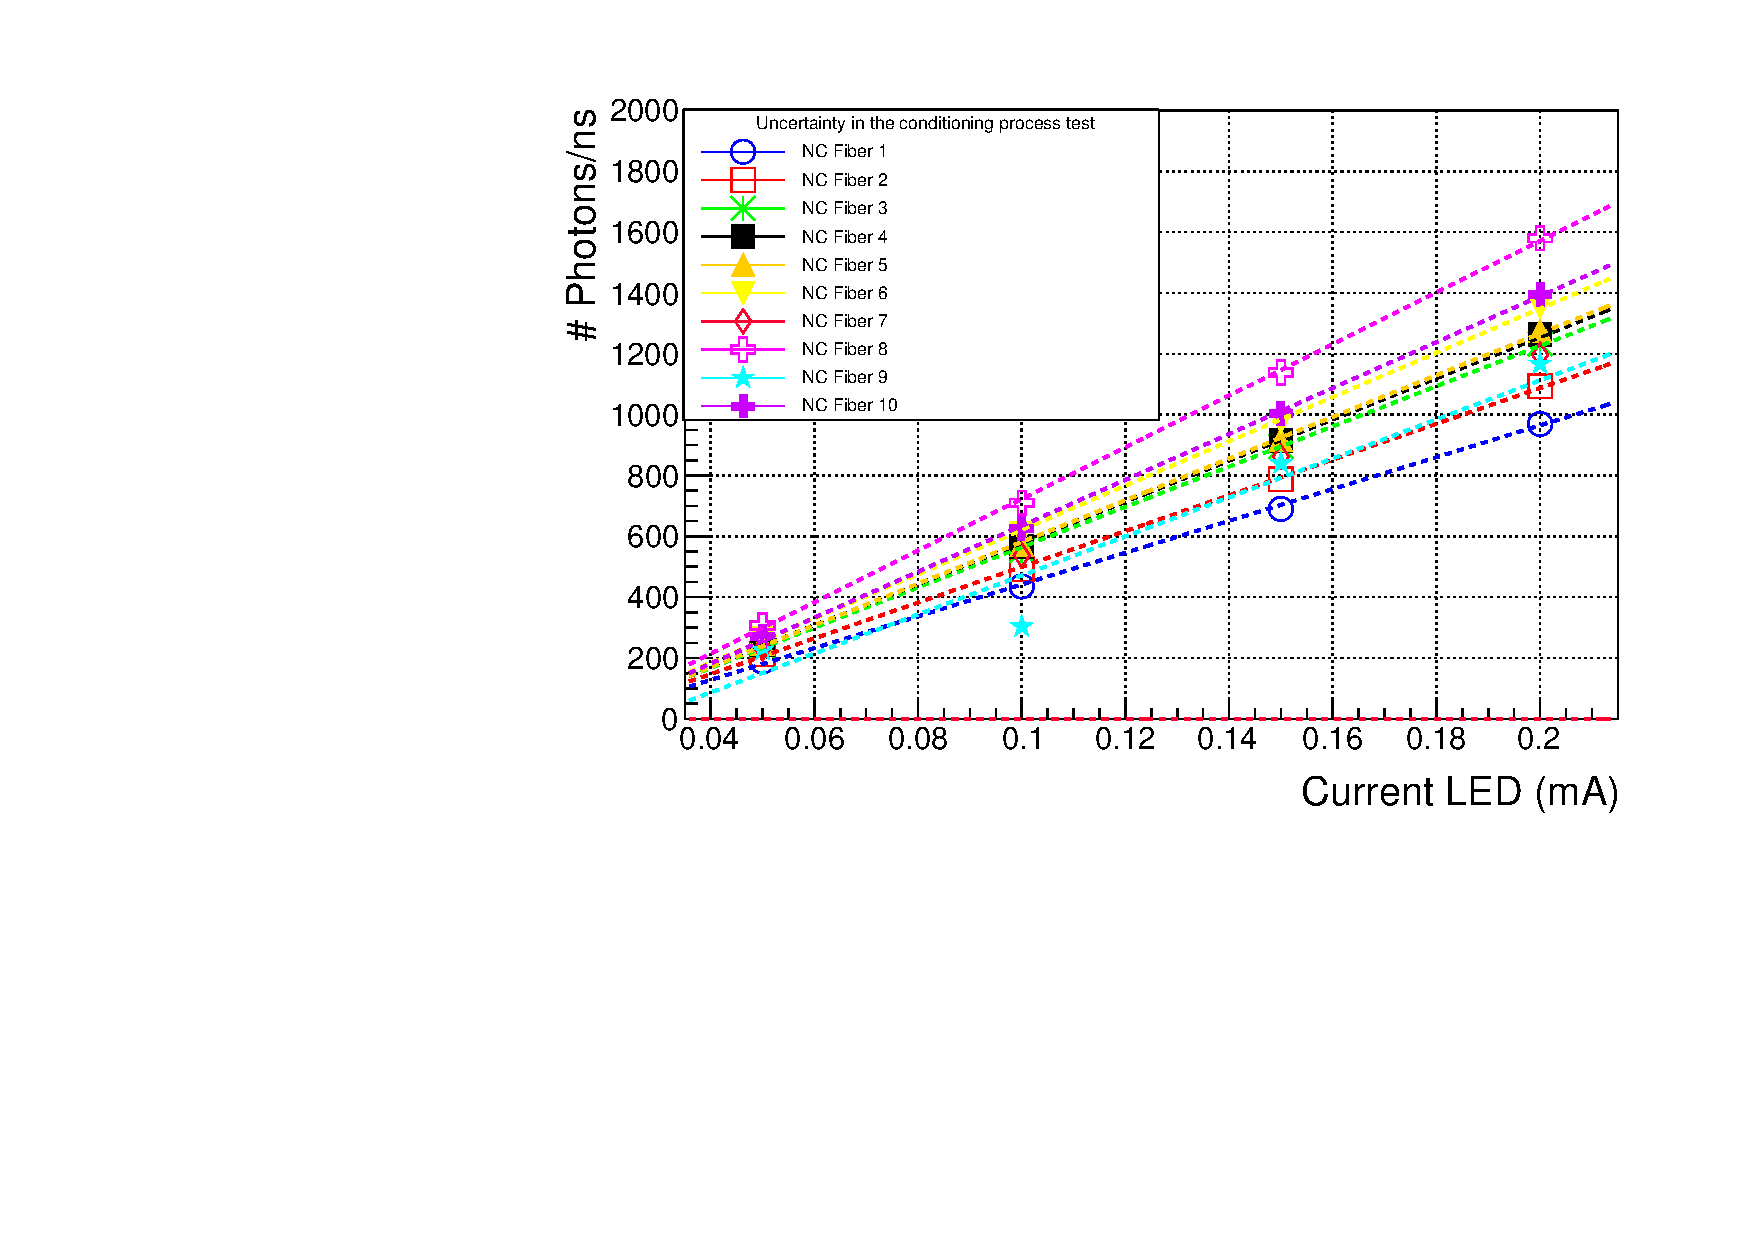
\includegraphics[scale=0.7]{4ResearchAndDevelopments/41Fibers/10_Different_samples_NoClad.pdf}
\caption{Number of photons/ns reaching the PMT for No Clad fibers.\label{fig:10samplesNC}}
\end{figure}

\begin{figure}[htbp]
 \centering
  %\subfloat[Number of photons/ns reaching the PMT for No Clad fibers.]{
   %\label{subfig:10samplesNC}
    %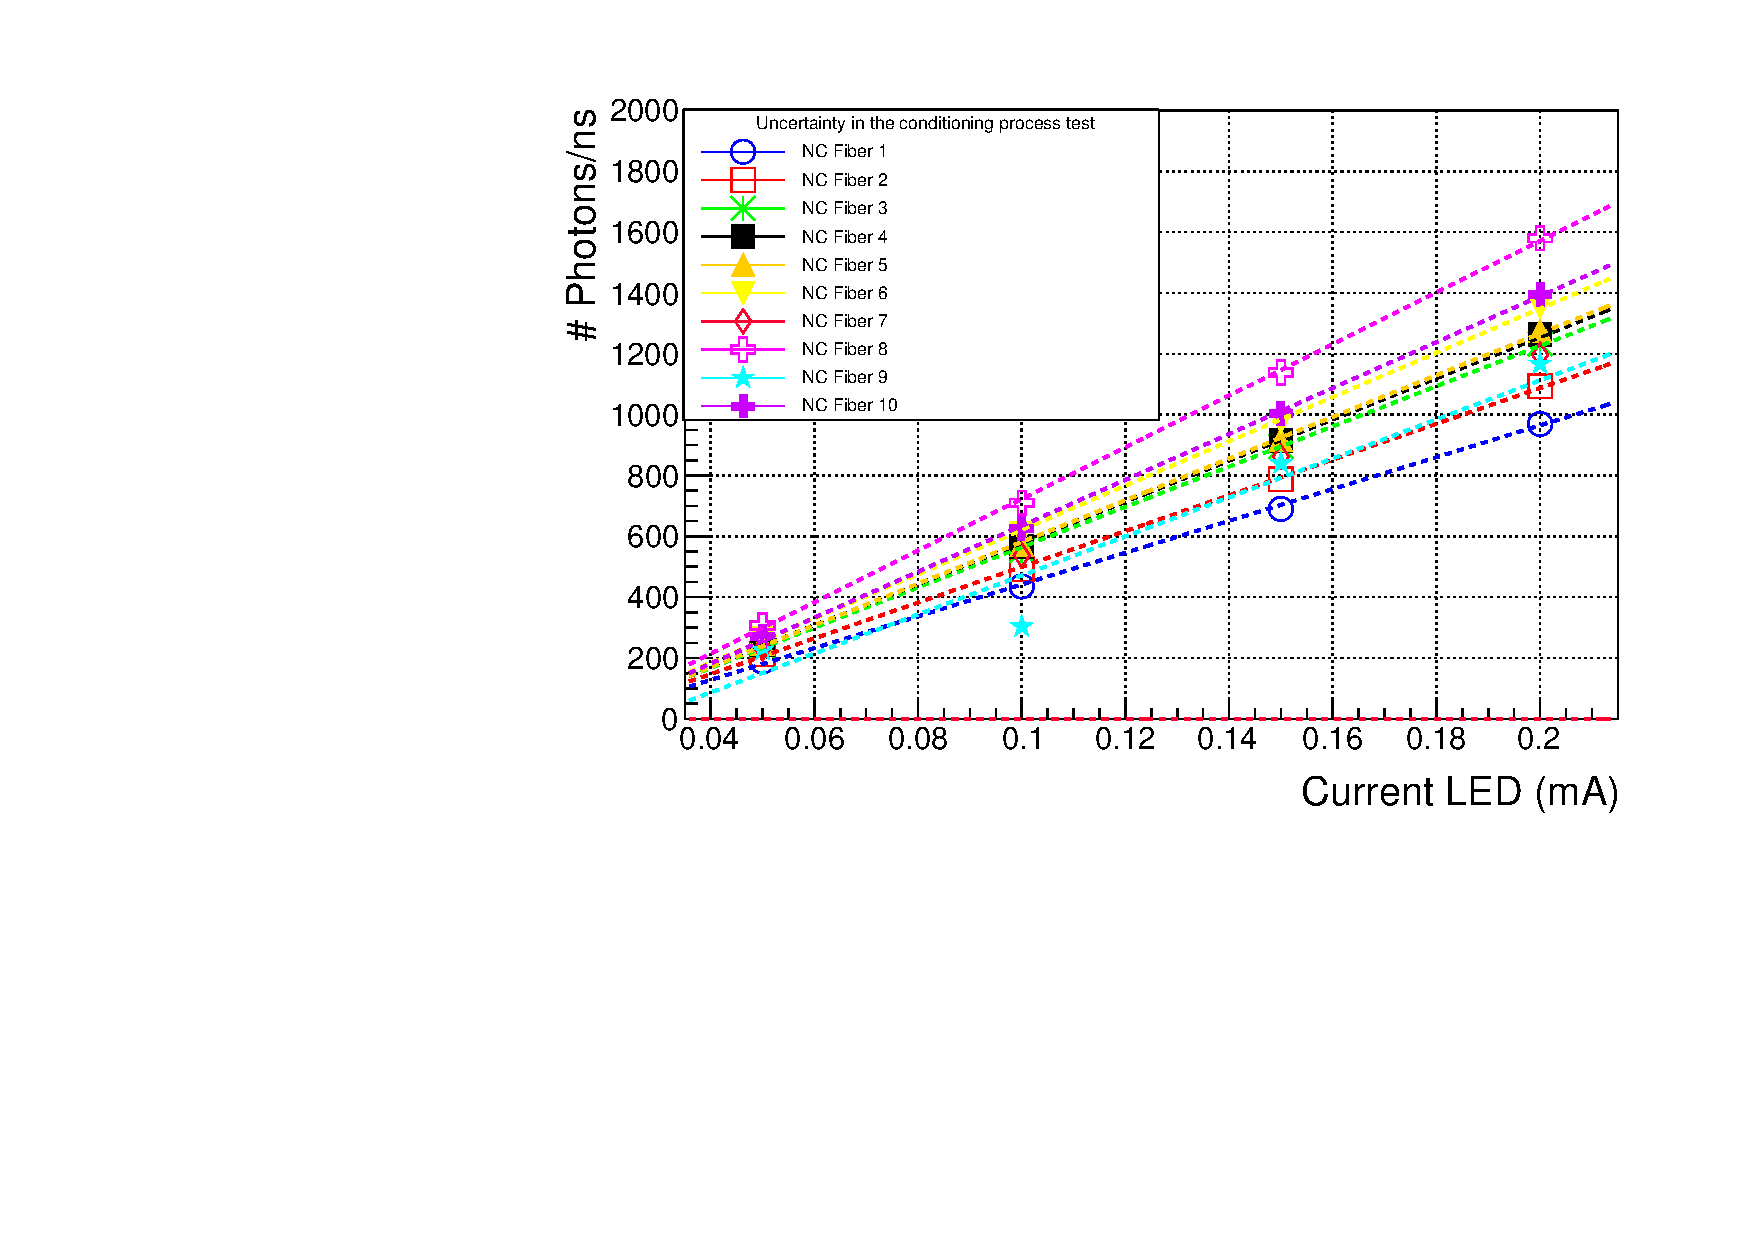
\includegraphics[width=0.75\textwidth]{4ResearchAndDevelopments/41Fibers/10_Different_samples_NoClad.pdf}}
    %\newline
  \subfloat[Number of photons/ns reaching the PMT for Single Clad fibers.]{
   \label{subfig:10samplesSC}
    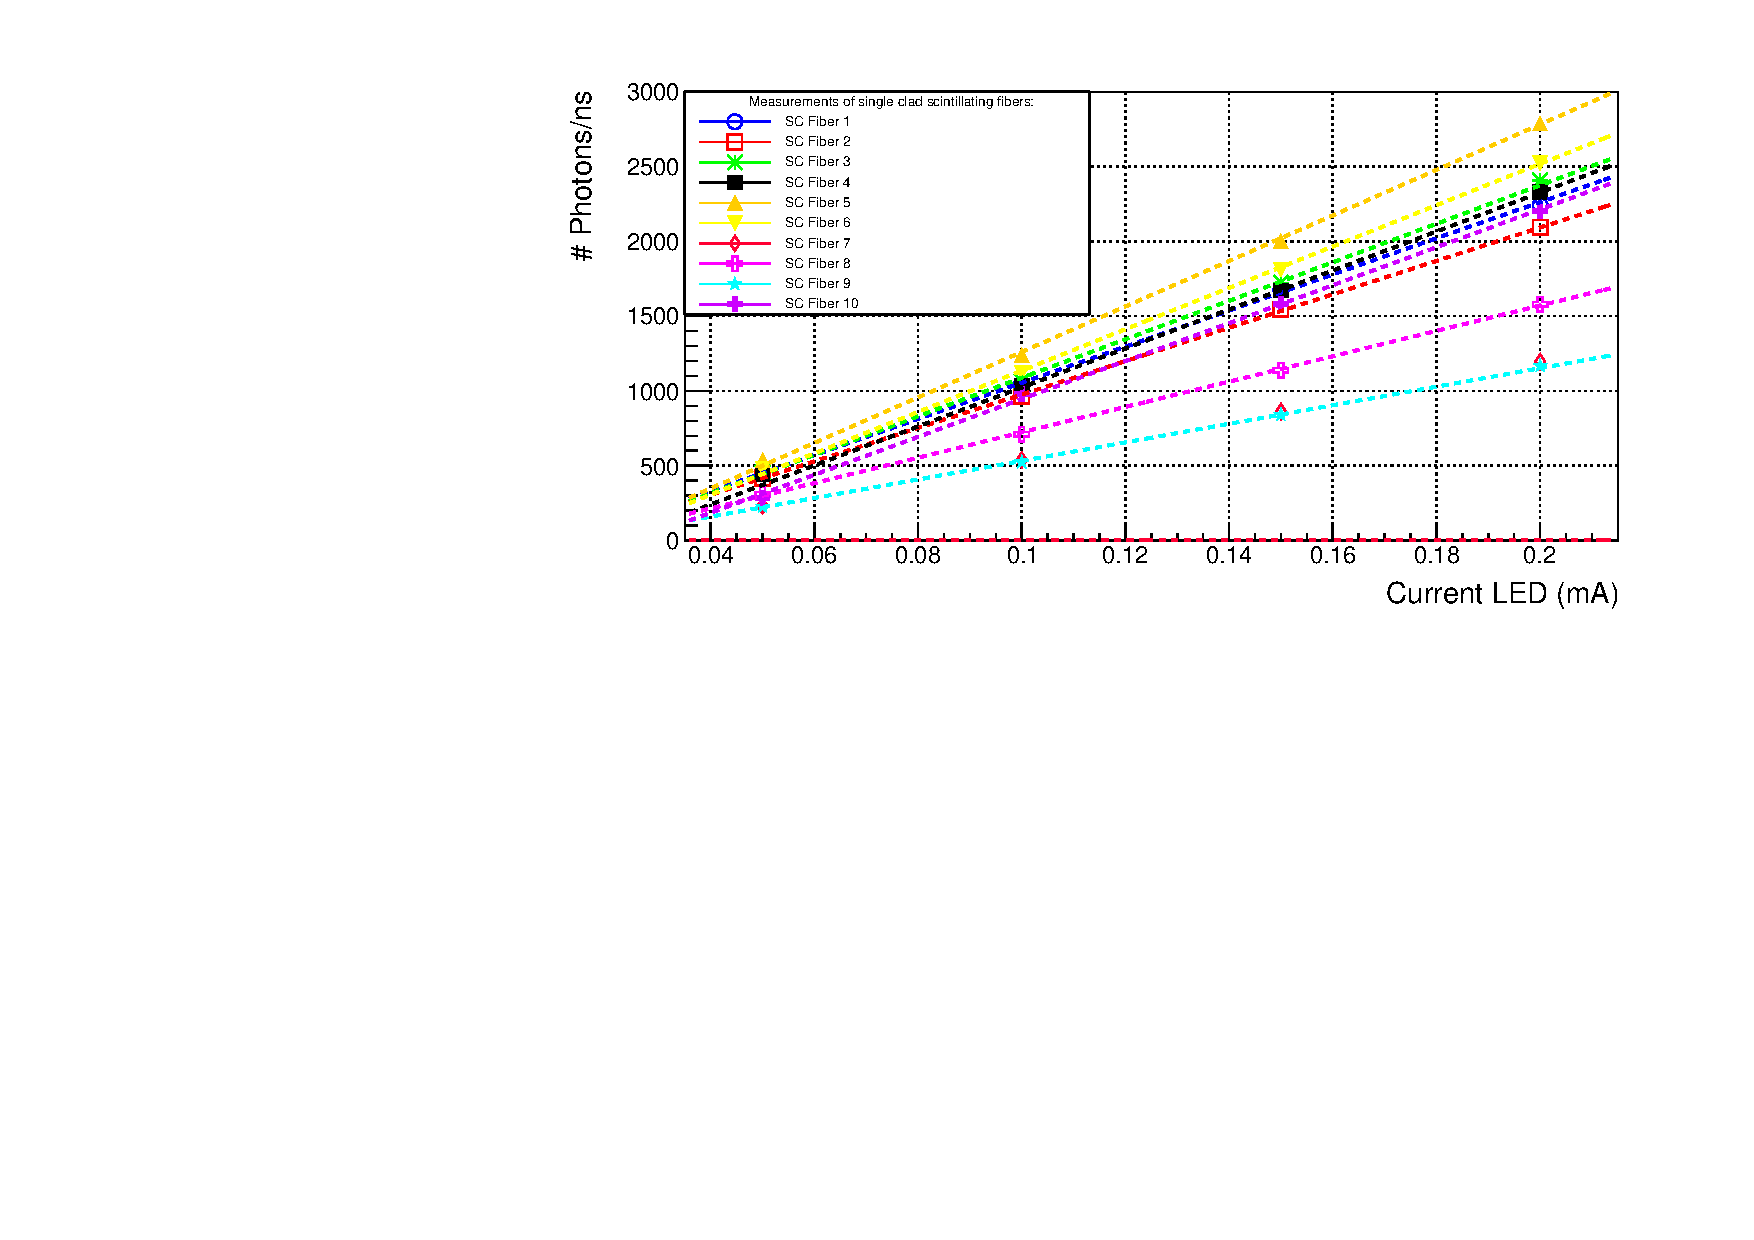
\includegraphics[width=0.9\textwidth]{4ResearchAndDevelopments/41Fibers/10_Different_samples_SingleClad.pdf}}
    \newline
    \subfloat[Number of photons/ns reaching the PMT for MultiClad fibers.]{
   \label{subfig:10samplesMC}
    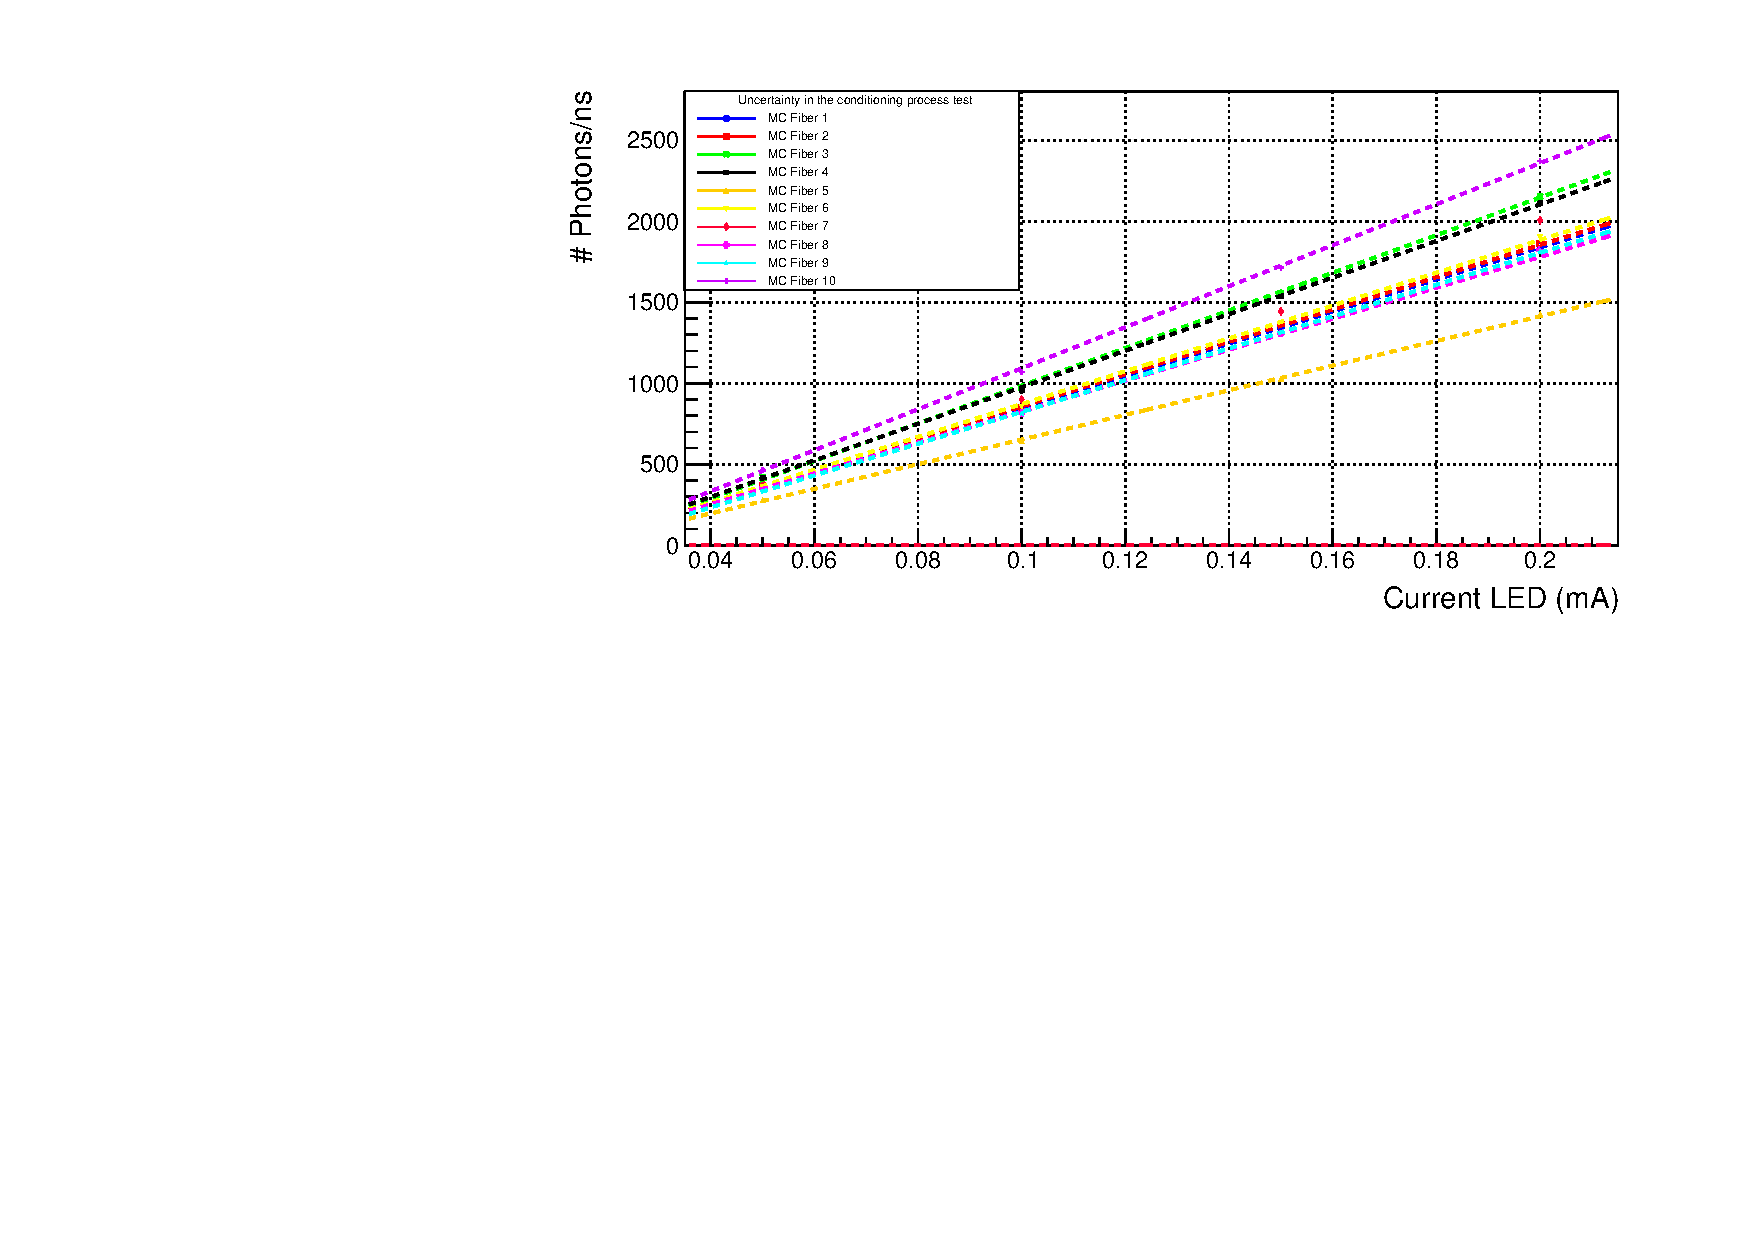
\includegraphics[width=0.9\textwidth]{4ResearchAndDevelopments/41Fibers/10_Different_samples_MultiClad.pdf}}    
 \caption{Number of photons/ns reaching the PMT for ten samples of each fibers type.}
 \label{fig:10samplesThreeTypes}
\end{figure}

The average of these 10 samples for each type of fibers and its standard deviation are summarized in Tables \ref{tab:10DifferentSamplesNoClad}, \ref{tab:10DifferentSamplesSingleClad} and \ref{tab:10DifferentSamplesMultiClad} and represented in Figure \ref{fig:AveregeThreeFiberTypes}, where they can be compared. 

\begin{table}[htbp]
%%\centering
\begin{center}
\begin{tabular}{|c|c|c|c|c|}
\hline
Led Int. (mA) & Average ($\gamma$/ns) & Std. Des. ($\gamma$/ns) & Rel. Std. Des. (\%)\\
\hline \hline \hline
$0.05$ & $243.46$ & $9.82$ & $4.03$ \\ \hline
$0.1$ & $540.62$ & $33.51$ & $6.20$ \\ \hline
$0.15$ & $902.74$ & $36.83$ & $4.08$ \\ \hline
$0.2$ & $1252.62$ & $50.48$ & $4.03$ \\ \hline
\end{tabular}
\caption{Average, standard deviation and relative standard deviation of 10 different samples of no clad fibers.}
\label{tab:10DifferentSamplesNoClad}
\end{center}
\end{table}

\begin{table}[htbp]
%%\centering
\begin{center}
\begin{tabular}{|c|c|c|c|c|}
\hline
Led Int. (mA) & Average ($\gamma$/ns) & Std. Des. ($\gamma$/ns) & Rel. Std. Des. (\%)\\
\hline \hline \hline
$0.05$ & $383.81$ & $33.23$ & $8.66$ \\ \hline
$0.1$ & $922.68$ & $73.97$ & $8.02$ \\ \hline
$0.15$ & $1485.10$ & $119.90$ & $8.07$ \\ \hline
$0.2$ & $2053.78$ & $166.39$ & $8.10$ \\ \hline
\end{tabular}
\caption{Average, standard deviation and relative standard deviation of 10 different samples of single clad fibers.}
\label{tab:10DifferentSamplesSingleClad}
\end{center}
\end{table}

\begin{table}[htbp]
%%\centering
\begin{center}
\begin{tabular}{|c|c|c|c|c|}
\hline
Led Int. (mA) & Average ($\gamma$/ns) & Std. Des. ($\gamma$/ns) & Rel. Std. Des. (\%)\\
\hline \hline \hline
$0.05$ & $376.68$ & $14.96$ & $3.97$ \\ \hline
$0.1$ & $870.87$ & $34.58$ & $3.97$ \\ \hline
$0.15$ & $1396.60$ & $55.24$ & $3.95$ \\ \hline
$0.2$ & $1932.57$ & $76.02$ & $3.93$ \\ \hline
\end{tabular}
\caption{Average, standard deviation and relative standard deviation of 10 different samples of multi clad fibers.}
\label{tab:10DifferentSamplesMultiClad}
\end{center}
\end{table}

\begin{figure}[h]
\centering
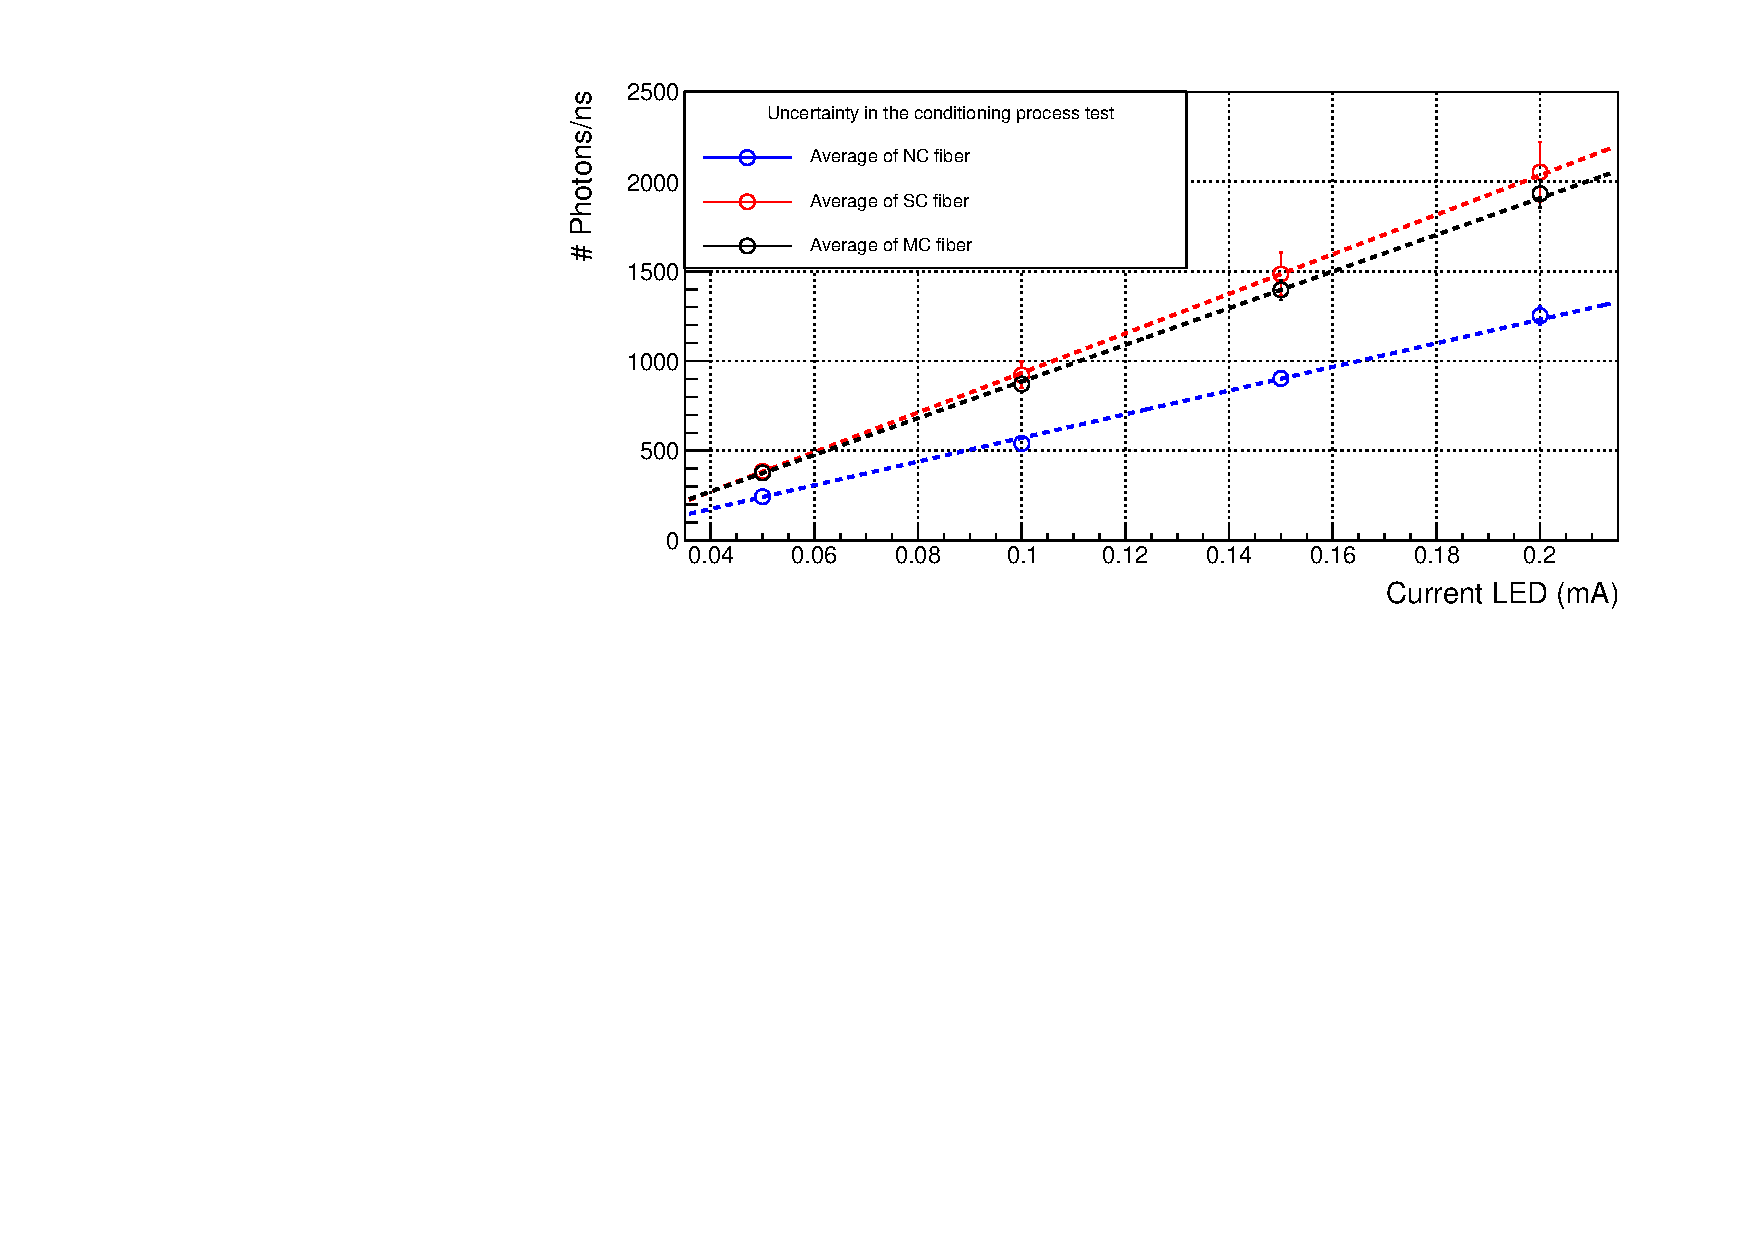
\includegraphics[scale=0.6]{4ResearchAndDevelopments/41Fibers/10_Different_Samples_Average_3_Fiber_Types.pdf}
\caption{Average of 10 samples for each fiber type (no clad, single clad and multiclad fibers).\label{fig:AveregeThreeFiberTypes}}
\end{figure}

As it is shown these figures, they have a very linear trent which confirms the correct behavior of the fibers. It can be appreciate that, similar to what happened with the previous test, single clad and multiclad fibers, both, have higher signals that no clad fibers, which means that the clad has an appreciable effect on the fiber collection efficiency and it could be a possible point for futur studies. 

Again, similar to what happened in the previous study, single-clad fibers have higher collection efficiency than multiclad fibers, something that was verified in all the tests performed.

The relative standard deviation are also presented in these tables, where we it can be seen that the dispersion of each fiber type for different LED intensities is practically negligible, which again verifies the correct behavior of the system. 

There is only one point (no clad fiber with $0.1~\milli\ampere $) that is higher than we expect. We can see in Table \ref{tab:10DifferentSamplesNoClad} that the reason for this is that its standard deviation is too high (as high as the measurement for no clad fibers with $0.15~\milli\ampere$). The reason was found in the sample 9, whose measurement was very different from the average, incresing the standard deviation, probably due to a problem in the measurement process. We discard this sample because this result is not representative.

To uniform the results, an average of these four values is calculated for each fiber type and shown in Table \ref{tab:RelativeStandardDeviations}, where the uncertainty in the fiber position and the uncertainty due to the conditioning process, previously calculated, are also shown. 

\begin{table}[htbp]
%%\centering
\begin{center}
\begin{tabular}{|c|c|c|c|}
\hline
Fiber type & $\sigma_t$ (\%) & $\sigma_{pos}$ (\%) & $\sigma_{con}$ (\%)\\\hline \hline \hline
No Clad & $4.01$ & $3.37$ & $2.17$ \\ \hline
Single Clad & $8.21$ & $2.17$ & $7.92$ \\ \hline
Multiclad & $3.96$ & $1.04$ & $3.82$ \\ \hline
\end{tabular}
\caption{Relative standard deviations ($\sigma_t$, $\sigma_{pos}$ and $\sigma_{con}$) measured in this test.}
\label{tab:RelativeStandardDeviations}
\end{center}
\end{table}

As it can be seen, the least uncertainty in the conditioning process is found in the no clad fibers, which means that the damage from this process occurs mainly in the fiber clad, which can be checked in Figure \ref{fig:ResultofPolishingProcess}. It was checked under the microscope that this damage only occurs at the end of the fiber.

Also, the largest relative standard deviation in this process is measured for single clad fibers, which means that the second clad increases the resistance of the fiber to this process.

In summary, this study has shown, on the one hand, the use of fiber clad improves the photon collection efficiency, which could be an interesting point for future studies, and, on the other hand, the relative statistical deviation due to the fiber conditioning process developed in the TRITIUM experiment was quantified for each fiber type, where it was checked that the main damage of the conditioning process is produced in the fiber clad so, if a method to create a clad for the fibers is developed, it should be applied after the fiber conditioning process.

Finally, the measurement of the photon collection efficiency of each type of fiber is shown. The collection efficiency is the percentage of photons collected along the fibers. It is usually given by the manufacturer per meter of fiber, $EC_ {100}$.

To measure it, we prepare ten different samples with a length of $10~\cm$ for each fiber type and measure each one using the set up previously explained. Then, the average and standard deviation was calculated using the equations \ref{eq:MeanAndStandardDesviation}, whose results are shown in Table \ref{tab:10DifferentSamplesAlltypes}.

\begin{table}[htbp]
%%\centering
\begin{center}
\begin{tabular}{|c|c|c|c|c|}
\hline
Led Int. (mA) & No clad ($\gamma$/ns) & Single clad ($\gamma$/ns) & MultiClad ($\gamma$/ns) \\
\hline \hline \hline
$0.05$ & $318.35 \pm 61.34$ & $549.62 \pm 70.79$ & $480.35 \pm 83.72$ \\ \hline
$0.1$ & $735.65 \pm 143.02$ & $1269.91 \pm 164.32$ & $1110.66 \pm 193.44$ \\ \hline
$0.15$ & $1183.91 \pm 232.07$ & $1983.93 \pm 230.97$ & $1777.40\pm 307.19$ \\ \hline
$0.2$ & $1645.18 \pm 323.76$ & $2506.97 \pm 208.01$ & $2338.43 \pm 350.24$ \\ \hline
\end{tabular}
\caption{Average and standard deviation of 10 different fibers of $10~\cm$.}
\label{tab:10DifferentSamplesAlltypes}
\end{center}
\end{table}

The collection efficiency can be calculated by comparing these tests with those performed for a fiber length of $20~\cm$, whose values has been previously shown in Tables \ref{tab:10DifferentSamplesNoClad}, \ref{tab:10DifferentSamplesSingleClad} and \ref{tab:10DifferentSamplesMultiClad} since both was made under the same conditions. The results is shown in Table \ref{tab:CollectionEfficiencyOfFibers}:


%Due to the reason that both tests were run in the same setup under exactly the same conditions, the difference between both situations is the photons per nanosecond that have not been collected in this extra $10~\cm$ of fiber. Therefore, using the equation \ref{}, the collection efficiency in $10~\cm$ of fiber can be calculated for each sort of fiber, whose result is shown in the last column.

\begin{table}[htbp]
%%\centering
\begin{center}
\begin{tabular}{|c|c|c|}
\hline
Fiber type & $CE_{10}$ (\%) & $CE_{100}$ (\%) \\\hline \hline \hline
No Clad & $75.97 \pm 7.61$ & $7.597 \pm 0.761$ \\ \hline
Single Clad & $77.96 \pm 5.66$ & $7.796 \pm 0.566$ \\ \hline
Multiclad & $82.60 \pm 7.24$ & $8.260 \pm 0.724$ \\ \hline
\end{tabular}
\caption{Collection efficiency of each fiber type for 10 centimeters, $CE_{10}$, and 1 meter, $CE_{100}$.}
\label{tab:CollectionEfficiencyOfFibers}
\end{center}
\end{table}

As the difference between the fiber length in both studies is only $10~\cm$, the collection efficiency calculated from these measurements, $CE_{10}$, is only at that distance. Assuming a linear dependence of this parameter with the distance, the value of $CE_{100}$ can be extrapolated.

The collection efficiency per meter given by the manufacturer Saint-Gobain is between 7\% and 3.44\% \cite{DataSheetBCF12Fiber}. As collimated photons are used in this study, it can be assumed that it is the best case, 7\%. 

As can be seen in Table \ref{tab:CollectionEfficiencyOfFibers}, our measured values are very close to the one provided by the manufacturer. The difference between this value for the three types of fiber studied is not as large as it was expected. A possible reason is that the difference in fiber length is only $10~\cm$ and it may not be enough to see this effect. It could be interesting to repeat these tests with a larger difference in fiber length.